\chapter{系统方案设计}

%系统架构图
\begin{figure}[htbp]
    \centering
    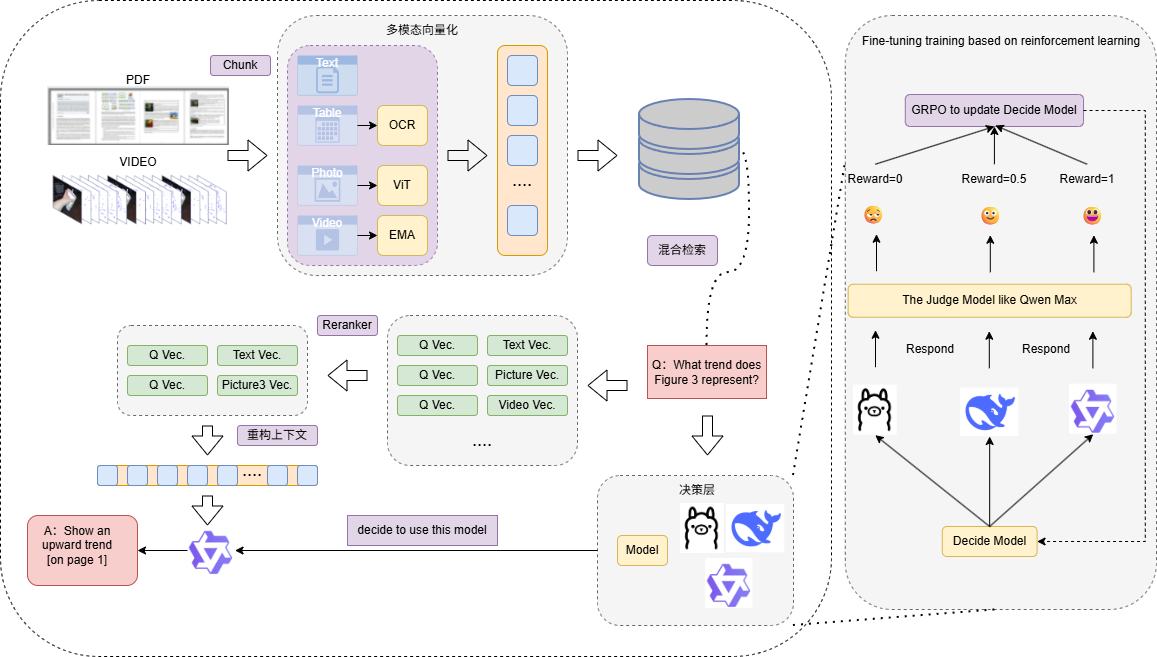
\includegraphics[width=0.95\textwidth]{image/frame.png}
    \caption{系统架构图}
    \label{fig:system_architecture}
\end{figure}


\section{系统架构}

\subsection{模型路由决策模块}

基于意图分类的前置决策层，采用强化学习自适应路由决策，使得系统能够选择最优的多模态模型来进行问答，在训练阶段让模型产生若干选择，然后让一个评测模型去评估答案，并给出分数，然后基于分数通过GRPO算法来更新路由模型的权重，使得路由模型能够逐渐学会在不同类型的问题上选择最合适的模型。

\subsection{多模态向量化}

在数据预处理阶段，首先需要通过版面分析将文档、截图或视频切块，并根据不同的模态，进行独立向量化。
\begin{itemize}
    \item \textbf{文本}：使用 BGE-m3 等模型对文本块向量化，形成基础索引。
    \item \textbf{表格}：使用 OCR 模型将表格转为 Markdown 等结构化格式，保留表格特征再向量化。
    \item \textbf{图片}：使用视觉编码模型ViT等提取图像特征并向量化，保留空间位置信息。
    \item \textbf{视频}：采用运动感知视频的MLLM，融合外观与时序运动特征以提升动作与场景理解，同时减少冗余的 token 数，降低显存占用。
\end{itemize}

\subsection{在线检索与决策}

\begin{itemize}
    \item \textbf{混合检索 (Hybrid Retrieval)}：同时搜索文本库、表格 Markdown 以及多模态视觉摘要关联的描述空间，获取 Top-K 初步召回片段。
    \item \textbf{Rerank重排序}：采用交叉编码器模型BGE-Reranker-v2-m3进行深度语义判断，二次打分筛选无关内容，降低干扰噪声，仅保留最相关的素材送入生成层。
\end{itemize}

\subsection{Generation生成阶段}

\begin{itemize}
    \item \textbf{上下文构建}：将检索到的文本、表格 Markdown 以及视觉元素的描述信息进行拼接，形成一个结构化且富含视觉线索的上下文输入。
    \item \textbf{VLM 多模态大模型推理}：将上下文输入到VLM中进行推理，生成结果，同时通过prompt设计引导模型在回答中明确标注引用的页码、图表来源等溯源信息。
\end{itemize}

\section{模型选择}

\begin{itemize}
    \item \textbf{Decide决策模型}：采用 Qwen-0.5B 等轻量模型，结合 GRPO 强化学习微调完成路由决策。
    \item \textbf{嵌入模型}
    \begin{itemize}
        \item \textbf{DeepSeek-OCR-2 OCR 模型}：专门针对文档中的视觉元素进行结构化处理，提取表格、图表等的特征信息。
        \item \textbf{BGE-Reranker-v2-m3 Reranker 模型}：在混合检索阶段对初步召回的文本和视觉描述进行二次打分，筛选出最相关的内容以供生成阶段使用。
    \end{itemize}
    \item \textbf{VLM 模型}： \textbf{Qwen2.5-VL }、\textbf{LLaMA 3.2 Vision}、\textbf{DeepSeek-VL}
\end{itemize}

\section{评测数据集与评测指标}

本项目在的评测数据集使用文档数据集\textbf{ DocVQA、ChartQA子集等}，如果未来时间允许的话，我们也会尝试用自建数据集的方式来进行评测，评测指标包括：

\begin{itemize}
    \item \textbf{评测检索与路由指标}：召回率（Recall@K），前 K 个重排中覆盖正确答案的比例与平均倒数排名 MRR
    \item \textbf{评测回答质量指标}： 均值归一化莱文斯坦相似度ANLS（DocVQA 官方标准指标）；精确匹配Exact Match (EM) 察系统对图表数据提取的精确度
    \item \textbf{溯源准确性}：统计输出引用是否确实指向相关知识，作为加分指标。
\end{itemize}